\PassOptionsToPackage{dvipsnames}{xcolor}
\documentclass[a4paper,11pt]{report} %article

\usepackage{graphicx,subfigure,afterpage,hyperref,xspace,xcolor,caption,soul,geometry,pdfpages,stackengine,eso-pic,fancyhdr,hyphenat,listings,longtable,url,enumitem,fancyvrb,textcomp}


%\usepackage[utf8]{inputenc} %to make the single quote appear correct after the encoding inserted above!

%command to substitute "{\em MyTaxyService}" with "\mts"
\newcommand{\mts}{\mbox{\normalfont\itshape myTaxiService}}
\geometry{margin=1in}

%header & footer style
\fancyhead{}
\fancyhead[C]{\iffloatpage{}{\slshape\rightmark}}
\fancyfoot{}
\fancyfoot[C]{\iffloatpage{}{\thepage}}
\renewcommand{\headrulewidth}{\iffloatpage{0pt}{0.4pt}}
\renewcommand{\footrulewidth}{\iffloatpage{0pt}{0.4pt}}
\pagestyle{fancy}
\renewcommand{\sectionmark}[1]{\markright{\thesection.\ #1}}
\renewcommand{\subsectionmark}[1]{\markright{\thesubsection.\ #1}}

%tOC style: sections bold 
\usepackage[subfigure]{tocloft}
\renewcommand{\cftsecfont}{\bfseries}
\renewcommand{\cftsecpagefont}{\normalfont\bfseries}% page numbers in bold
\renewcommand{\cftdotsep}{1}
\renewcommand{\cftsecleader}{\bfseries\cftdotfill{\cftsecdotsep}}% dot leaders in bold

%to keep the links of the TOC invisible
\hypersetup{
	colorlinks,
	citecolor=black,
	filecolor=black,
	linkcolor=black,
	urlcolor=black
}


\title{Politecnico di Milano\\A.A. 2015/2016\\Software Engineering 2\\ \bigskip 
Assignment 5: Project Plan\\
{\normalsize Version 1.0}}
\author{Alessandro Baldassari (mat. 841561) \\ Alberto Bendin (mat. 841734) \\ Francesco Giarola (mat. 840554)}


%to set the nested bullet lists style
\renewcommand{\labelitemii}{$\circ$}
%\renewcommand{\labelitemii}{}
\renewcommand{\labelitemiii}{$\diamond$}

%to avoid the hyphenation of the name of the software
\hyphenation{myTaxyService}

\begin{document}
	
	%fIRSTPAGE
	
	%pOLIMI-LOGO
	\begin{figure}[t]
		\centering
		\includegraphics[width=1\linewidth]{"Pictures/polimi-logo"}
		\label{fig:polimi-logo}
	\end{figure}
	
	\maketitle
		
	
	%bLANK-PAGE
	\thispagestyle{empty}
	\clearpage\mbox{}\clearpage

	
	
	
	%to number the section from 1 instead of 0.1 with the report class, without using the article class. Avoid the forced use of chapters to number from 1. Tailored for REPORT class!!!
	\renewcommand*\thesection{\arabic{section}}
	\renewcommand*\thesubsection{\arabic{section}.\arabic{subsection}}
	\renewcommand*\thesubsubsection{%
	\arabic{section}.\arabic{subsection}.\arabic{subsubsection}%
	}
	\setcounter{secnumdepth}{4}
	\setcounter{tocdepth}{4}
	

	
	%to change the page numbering from roman in the toc to arabic
	\pagenumbering{roman}
	\tableofcontents
	\newpage
	\pagenumbering{arabic}
	
	
	%to insert the writing "Page" above page numbers in the TOC
	\addtocontents{toc}{~\hfill\textrm{Page}\par}
	
	%tables style
	\renewcommand{\arraystretch}{1.2}
	\setlength{\tabcolsep}{12pt}
	
	\section{Introduction} 
		\subsection{Purpose and Scope}
			The main purpose of the project plan is to plan time, cost and resources adequately to estimate the work needed and to effectively manage risk during project execution. A failure to adequately plan reduces the project's chances of successfully accomplishing its goals.\smallskip\\
			Project planning generally consists of:
			\begin{itemize}
				\item Identifying deliverables and creating the work breakdown structure;
				\item Identifying the activities needed to complete those deliverables and networking the activities in their logical sequence;
				\item Estimating the resource requirements for the activities;
				\item Estimating time and cost for activities;
				\item Developing the schedule;
				\item Developing the budget;
				\item Resource allocation (organization of work loads);
				\item Risk planning.
			\end{itemize} 
			This document is based on an analysis made with two different algorithmic metrics of the system for \mts{}. The first one is the Function Points (FP), which is used to estimate the software dimension (code size), which is directly used to evaluate the cost. The second is the COCOMO II that is used to estimate the efforts required in the development of a project by taking in account: characteristics of people, products and process. 
			
		\subsection{List of Definitions and Abbreviations}
			The following acronyms are used in this document:
			\begin{itemize}
				\item FP: Function Points
				\item COCOMO: COnstructive COst MOdel
				\item ILF: Internal Logic File
				\item EIF: External Interface File
				\item PM: Person-Months
				\item SLOC: Source Lines of Code
				\item KSLOC: Thousands of SLOC
				\item SD: Scale Drivers
			\end{itemize}
			The following definitions are used in this document:
			\begin{itemize}
				\item Deliverables: are work that are delivered to the customer, e.g. a requirement document for the system.
			\end{itemize}
	
	\pagebreak		
	\section{Function Point analysis}
		\subsection{Introduction}
			The Function Point estimation approach is based on the amount of functionalities in a software and their complexity. Indeed the effort to develop a software project grows with the number of external inputs and outputs, user interactions, files and interfaces used by the system; therefore a weight is associated to all these functionalities and the total effort is computed summing all the partial values.\bigskip \\
			The parameters used to perform this estimation are summarized in the following tables, taken from COCOMO II, Model Definition Manual at:\smallskip\\ \href{http://csse.usc.edu/csse/research/COCOMOII/cocomo2000.0/CII\_modelman2000.0.pdf}{http://csse.usc.edu/csse/research/COCOMOII/cocomo2000.0/CII\_modelman2000.0.pdf}\bigskip\\
%			This first schema is used to determine the complexity-level function counts. It classifies each functionality into Low, Average and High complexity levels.\smallskip\\
%			\begin{minipage}{\linewidth}
%				%			\vspace*{-0.35cm}
%				\makebox[\linewidth]{
%					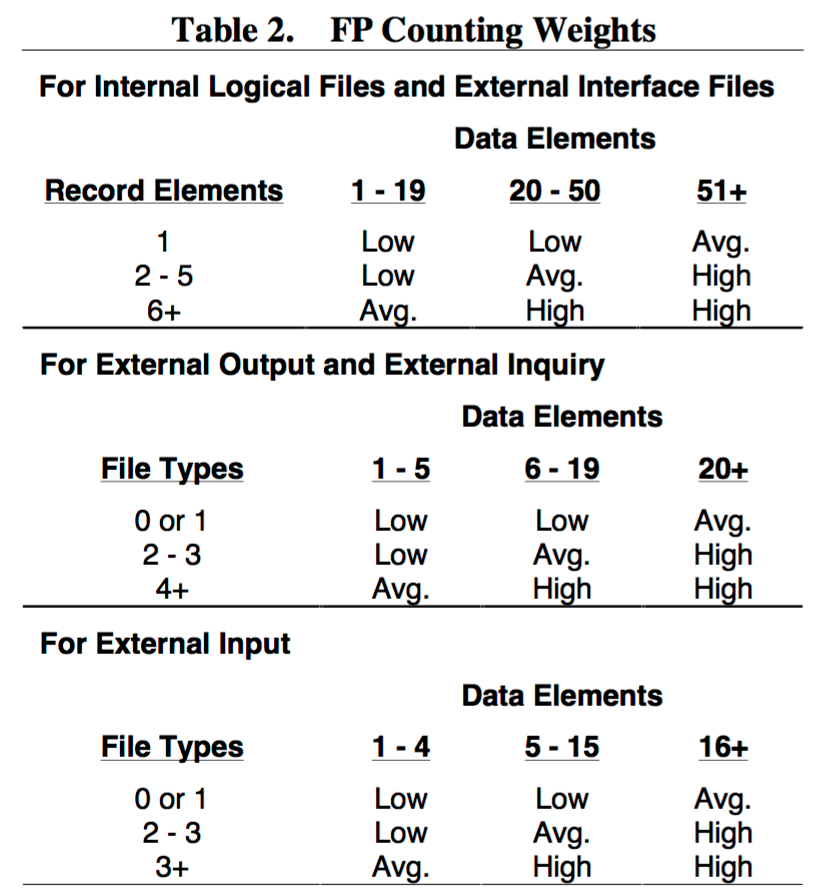
\includegraphics[keepaspectratio=true,scale=0.3]{Pictures/TableComplexity.png}}
%			\end{minipage}		
%			\bigskip\\
%			\smallskip\\
			The schema below defines the weights assigned to every level of complexity for all the FP types.\smallskip\\
			\begin{minipage}{\linewidth}
				%			\vspace*{-0.35cm}
				\makebox[\linewidth]{
					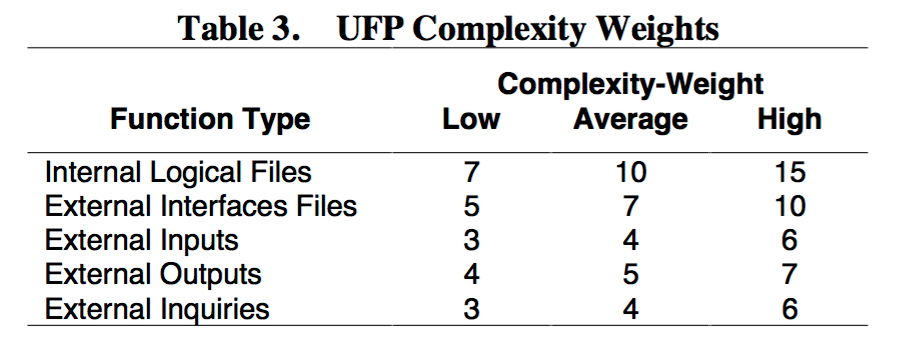
\includegraphics[keepaspectratio=true,scale=0.3]{Pictures/TableWeights.png}}
			\end{minipage}
			\bigskip\\
			Here is a brief explanation of the FP types:
			\begin{itemize}
				\item Internal Logic File: homogeneous set of data used and managed by the application
				\item External Interface File: homogeneous set of data used by the application but generated and maintained by other applications
				\item External Input: elementary operation to elaborate data coming from the external environment
				\item External Output: elementary operation that generates data for the external environment (it usually includes the elaboration of data from logic files)
				\item External Inquiry: Elementary operation that involves input and output (without significant elaboration of data from logic files)
				
			\end{itemize}
	
		\subsection{FP types estimation}
			\begin{itemize}
				\item ILF
							\renewcommand{\arraystretch}{1.2}
							\setlength{\tabcolsep}{12pt}
					\begin{center}
						\begin{tabular}{| p{7cm} | p{2.5cm} | p{2cm} |}\hline
							\textbf{Functionalities} & \multicolumn{1}{|c|}{\textbf{Complexity}} & \textbf{FP Count}\\\hline
							Users & \multicolumn{1}{|c|}{Simple} & \multicolumn{1}{|c|}{7}\\\hline
							Ride & \multicolumn{1}{|c|}{Complex} & \multicolumn{1}{|c|}{15}\\\hline
							Request & \multicolumn{1}{|c|}{Medium} & \multicolumn{1}{|c|}{10}\\\hline		
							Zone & \multicolumn{1}{|c|}{Medium} & \multicolumn{1}{|c|}{10}\\\hline	
							Taxi & \multicolumn{1}{|c|}{Simple} & \multicolumn{1}{|c|}{7}\\\hline		
							Payment-Receipts & \multicolumn{1}{|c|}{Simple} & \multicolumn{1}{|c|}{7}\\\hline																														
							\multicolumn{2}{|l|}{Total:} & \multicolumn{1}{|c|}{56}\\\hline
						\end{tabular}
					\end{center}
				\item EIF
				\renewcommand{\arraystretch}{1.2}
				\setlength{\tabcolsep}{12pt}
				\begin{center}
					\begin{tabular}{| p{7cm} | p{2.5cm} | p{2cm} |}\hline
						\textbf{Functionalities} & \multicolumn{1}{|c|}{\textbf{Complexity}} & \textbf{FP Count}\\\hline						
						Payment Data & \multicolumn{1}{|c|}{Medium} & \multicolumn{1}{|c|}{7}\\\hline
						Google Maps & \multicolumn{1}{|c|}{Medium} & \multicolumn{1}{|c|}{7}\\\hline
						Push notification metadata & \multicolumn{1}{|c|}{Simple} & \multicolumn{1}{|c|}{5}\\\hline		
						\multicolumn{2}{|l|}{Total:} & \multicolumn{1}{|c|}{19}\\\hline	
					\end{tabular}
				\end{center}
				\item Ext. INPUT
				\renewcommand{\arraystretch}{1.2}
				\setlength{\tabcolsep}{12pt}
				\begin{center}
					\begin{tabular}{| p{7cm} | p{2.5cm} | p{2cm} |}\hline
						\textbf{Functionalities} & \multicolumn{1}{|c|}{\textbf{Complexity}} & \textbf{FP Count}\\\hline
						Login & \multicolumn{1}{|c|}{Simple} & \multicolumn{1}{|c|}{3}\\\hline
						SignUp & \multicolumn{1}{|c|}{Simple} & \multicolumn{1}{|c|}{3}\\\hline
						Create request & \multicolumn{1}{|c|}{Simple} & \multicolumn{1}{|c|}{3}\\\hline					
						Pay & \multicolumn{1}{|c|}{Medium} & \multicolumn{1}{|c|}{4}\\\hline		
						Delete request & \multicolumn{1}{|c|}{Complex} & \multicolumn{1}{|c|}{6}\\\hline	
						Set taxi availability & \multicolumn{1}{|c|}{Simple} & \multicolumn{1}{|c|}{6}\\\hline					
						Accept/reject ride request & \multicolumn{1}{|c|}{Simple} & \multicolumn{1}{|c|}{3}\\\hline			
						Update taxi position & \multicolumn{1}{|c|}{Simple} & \multicolumn{1}{|c|}{3}\\\hline				
						Managers taxi drivers & \multicolumn{1}{|c|}{Medium} & \multicolumn{1}{|c|}{4}\\\hline				
						Create ride & \multicolumn{1}{|c|}{Complex} & \multicolumn{1}{|c|}{6}\\\hline		
						Allocate taxi & \multicolumn{1}{|c|}{Complex} & \multicolumn{1}{|c|}{6}\\\hline																																																												
						\multicolumn{2}{|l|}{Total:} & \multicolumn{1}{|c|}{44}\\\hline
					\end{tabular}
				\end{center}
				\item Ext. INQUIRY
				\renewcommand{\arraystretch}{1.2}
				\setlength{\tabcolsep}{12pt}
				\begin{center}
					\begin{tabular}{| p{7cm} | p{2.5cm} | p{2cm} |}\hline
						\textbf{Functionalities} & \multicolumn{1}{|c|}{\textbf{Complexity}} & \textbf{FP Count}\\\hline
						Request history & \multicolumn{1}{|c|}{Simple} & \multicolumn{1}{|c|}{3}\\\hline
						Manage profile & \multicolumn{1}{|c|}{Simple} & \multicolumn{1}{|c|}{3}\\\hline
						Ride history & \multicolumn{1}{|c|}{Simple} & \multicolumn{1}{|c|}{3}\\\hline		
						Public API & \multicolumn{1}{|c|}{Medium} & \multicolumn{1}{|c|}{4}\\\hline	
						DB & \multicolumn{1}{|c|}{Medium} & \multicolumn{1}{|c|}{4}\\\hline		

						\multicolumn{2}{|l|}{Total:} & \multicolumn{1}{|c|}{17}\\\hline
					\end{tabular}
				\end{center}
				\item Ext. OUTPUT
				\renewcommand{\arraystretch}{1.2}
				\setlength{\tabcolsep}{12pt}
				\begin{center}
					\begin{tabular}{| p{7cm} | p{2.5cm} | p{2cm} |}\hline
						\textbf{Functionalities} & \multicolumn{1}{|c|}{\textbf{Complexity}} & \textbf{FP Count}\\\hline
						SMS & \multicolumn{1}{|c|}{Medium} & \multicolumn{1}{|c|}{4}\\\hline
						Email & \multicolumn{1}{|c|}{Simple} & \multicolumn{1}{|c|}{4}\\\hline
						PushNotification & \multicolumn{1}{|c|}{Simple} & \multicolumn{1}{|c|}{4}\\\hline		
						Zone & \multicolumn{1}{|c|}{Simple} & \multicolumn{1}{|c|}{10}\\\hline																						
						\multicolumn{2}{|l|}{Total:} & \multicolumn{1}{|c|}{17}\\\hline
					\end{tabular}
				\end{center}																	
			\end{itemize}	
			The total number of FPs it then 153.
	
	\section{COCOMO II analysis}
		\subsection{Introduction}	
			This estimation is achieved through a complex, statistical model that takes in account the characteristics of the product but also of people and process. The result of this technique is the estimation of Person-Months required to develop the project.\\
			The COCOMO II calculations are based on the estimated of the software dimension in source lines of code (SLOC).
	
	\section{Tasks identification and schedule}	
	
	\section{Resources allocation}	
	
	\section{Risk planning and management}	

	\pagebreak
	\section{References}
		Material from Wikipedia
		\begin{itemize}
			\item Project management: \href{https://en.wikipedia.org/wiki/Project\_management\#Planning}{https://en.wikipedia.org/wiki/Project\_management\#Planning}
		\end{itemize}
	
	\section{Appendix}
		\subsection{Software and tools used}
		\begin{itemize}
			\item TeXstudio 2.10.6 (\href{http://www.texstudio.org/}{http://www.texstudio.org/}) to redact and format this document.
			\item Astah Professional 7.0 (\href{http://astah.net/editions/professional}{http://astah.net/editions/professional}) 
		\end{itemize}
		
		\subsection{Hours of work} The time spent to redact this document:
		\begin{itemize}
			\item Baldassari Alessandro: 12 hours.
			\item Bendin Alberto: 12 hours.
			\item Giarola Francesco: 12 hours.
		\end{itemize}

\end{document}